\chapter{Background}
\label{chapter:background}

This chapter gives an overview on the theoretical background of scans and what
is needed to make them efficient on modern hardware. Then some possible
solutions are introduced and the approaches that are evaluated later in this
thesis are described in detail.

\section{Memory}

Since main memory has become large and cheap enough to store very large data
sets, many database systems no longer bother reading data from slower but
cheaper storage such as hard drives, but keep everything in main memory and
perform all queries directly there. This lead to database systems that are much
faster than the previous generation of database systems. However, there are
performance limitations to this approach: it is a well-known fact that processor
performance is growing much faster than memory performance is growing, as
illustrated in Figure~\ref{fig:memorywall}.

\begin{figure}[h] \begin{center}
\begin{tikzpicture} \begin{semilogyaxis}[
  grid,
  width=0.8*\textwidth,
  xlabel=Year,
  ylabel=Normalized Performance,
  xmin=1978, xmax=2010,
  ymax=100000,
  scaled ticks=false,
  log ticks with fixed point,
  x tick label style={/pgf/number format/fixed,
                      /pgf/number format/min exponent for 1000 sep=5},
  legend columns=-1,
  legend entries={CPU Performance (SPECint), DRAM Latency},
  legend to name=leg:memorywall,
]
\addplot+ table[header=false] {data/hennessy_cpu.csv};
\addplot+ table[header=false, y expr=250/\thisrowno{1}] {data/hennessy_ramcycles.csv};
\end{semilogyaxis}
\end{tikzpicture}
\ref*{leg:memorywall}
\end{center}
\caption{CPU and DRAM performance over time~\cite{hennessyarch}.}
\label{fig:memorywall}
\end{figure}

This performance discrepancy has been growing over time and is unlikely to
change in the near future. The effect is mainly due to the used type of memory,
so-called dynamic RAM (DRAM), which is extremely dense in terms of on-chip space
and can thus be produced very cheaply. However, it relies on charging and
discharging of capacitors, which is comparatively slow: reading a single bit from
DRAM can take hundreds of processor cycles. Processors use faster static RAM in
small caches which store data that was recently accessed. This principle of
locality helps performance in programs working on small data sets but for the
large data sets typically used in database systems it rarely makes a difference,
because caches are too small to hold all of the data.

To overcome expensive one-bit reads, many bits are read from RAM in parallel,
hiding the time needed to charge and discharge the capacitors. This essentially
means that a block of memory is read in the same amount of time as a single bit
is. To further improve the access times, the CPU detects sequential access of a
block of memory and will instruct the memory controller to load the next blocks
in advance. Because the next block is read in the background the latency is
invisible to the user. This so-called prefetching strategy is the only way high
bandwidth can be achieved with this kind of dynamic memory. Common methods to
accelerate accesses in database systems, such as trees and hash tables, use a
memory access pattern that cannot take advantage of prefetching, so a different
approach is needed.

\section{SIMD}

The idea behind SIMD (Single Instruction/Multiple Data) architectures as
first classified by Flynn \cite{flynnsimd}, is to use a single instruction
stream to process many different values at once. The earliest members of this
class of architectures were the vector processors of the 1970's such as the
Cray 1 or the Earth Simulator, the fastest supercomputer in the world in the year
2002 \cite{hennessyarch}. In a vector processor the size of a register is not
static but the number of elements in a register can be configured at runtime up
to a certain limit. The Cray 1 had a limit of 64 values in a register, each of
the values 64 bits wide. When arithmetic instructions are executed with such a
vector register, the individual values in the operands can be processed in
parallel as far as resources permit. So processing a 64-element vector can take
significant less than 64 cycles. Load operations typically gather values that
can be scattered throughout memory into a single register and load operations
have to disperse the values back into memory. By this approach a CPU with a vector
instruction set can perform the same operations while executing dramatically
fewer instructions than an architecture that operates on a single value at a
time. This frees up instruction decoding resources that can be repurposed to
increase throughput elsewhere.

However, classic vector architectures have not become the most prevalent model
for modern processor architectures, obvious reasons being:
\begin{itemize}
\item Superscalar out-of-order processors already provide parallelism by
automatically identifying independent instructions and executing them
simultaneously.
\item Gathering loads and scattering stores are not a good fit for caches and
memory organized in fixed-size blocks where at least a full block is fetched or
stored. This would waste a significant amount of memory bandwidth and cache
memory.
\item The large variable-length registers add additional state to the processor.
This state must be managed by the operating system, making the switching between
processes more expensive.
\end{itemize}

In the end, a fairly limited subset of a vector processor's instruction set has
found its way into the instructions set of virtually any commodity processor,
except those that are geared towards low-performance embedded applications.
These so-called multimedia instructions only support fixed-size registers which
can usually be overlaid with different data types. For example registers
containing 128 bits can be used as either four 32-bit values or eight 16-bit
values. This means there are many different instructions compared to the
approach taken by vector architectures.  Scattering and gathering is usually not
present or only in a limited form by loading values separated by a constant gap.
Examples for this form of vector instructions are MMX, SSE and AVX on Intel
CPUs, AltiVec on PowerPC or NEON on ARM processors.

To understand why SIMD still provides an advantage over superscalar
instruction-level parallelism the latency and throughput of normal instructions
has to be taken into account. In Table~\ref{tab:latencies} the latencies and
throughput for loads and additions are shown. Now imagine a loop creating a sum
over 32-bit values; requiring a load and an add. All instructions are fully
pipelined, so we can load two 32-bit integers and perform two additions per
cycle, the full throughput is not achievable, because we cannot load more than
two values. Now we change the loop to work on 256-bit vectors, the load
throughput does not change with size, so we can load 16 32-bit integers per cycle
and still perform 2 full adds, adding all 16 integers. In theory we now
increased the throughput eightfold. In practice the performance will be bound by
memory latency though, unless the number of arithmetic instructions is
increased.

\begin{table}\center
\begin{tabular}{c|c|c}
Instruction & Latency & Throughput\\
\hline
Scalar load & (depends on cache) & 2 per cycle\\
Scalar add & 1 cycle & 4 per cycle\\
%Scalar mul & 3 cycles & 1 per cycle\\
Vector load & (depends on cache) & 2 per cycle\\
Vector add & 1 cycle & 2 per cycle\\
%Vector mul & 5 cycles & 1 per cycle
\end{tabular}
\caption{Instruction latencies and throughput on Intel Haswell \cite{agnertables}}
\label{tab:latencies}
\end{table}

\newpage
\section{Scans}

One of the most basic primitives to build a database system is the scan. For a
given table in the database the scan compares every row against a given
predicate and returns which rows match that predicate. This is equivalent to a
linear search over a block of memory, the runtime is $\mathcal{O}(n)$, where $n$
is the number of rows.

For a long time, scans were regarded as something to avoid in database systems.
Index data structures were developed to accelerate accessing the database. For
example, evaluating the predicate $a < x < b$ on a sorted table or binary tree
can be done in two $\mathcal{O}(\log n)$ binary searches. On the first glance
this should be a lot faster than the na\"ive $\mathcal{O}(n)$ scan, but a binary
search has a number of downsides.

\begin{itemize}
  \item Keeping sorted data available requires redundancy or expensive data
    movement during modification operations. The indexes also need to be
    maintained after every change to the underlying data.
  \item A binary search executes $\mathcal{O}(\log n)$ branch instructions,
    every single branch is dependent on the input data and not predictable.
    Mispredicted branches slow down the scan as the processor has to wait on the
    result before proceeding with the next value.
  \item Most importantly, binary searches introduce random access to the data
    instead of a sequential access pattern. When the data does not fit into
    cache, every access has to pay the full access time of the DRAM and cannot
    use the prefetching to hide memory latency described above.
\end{itemize}

The other major indexing technique, hashing, can avoid branching. It still
requires redundancy and uses a random memory access pattern. It is obvious that
neither binary search nor hashing can take advantage of fast sequential accesses
for databases in DRAM on modern hardware. Of course the actual performance
depends among other things on the data distribution and the percentage of values
selected during the scan, so there are still use cases where an index is highly
preferable.

\begin{figure}[h] \begin{center}
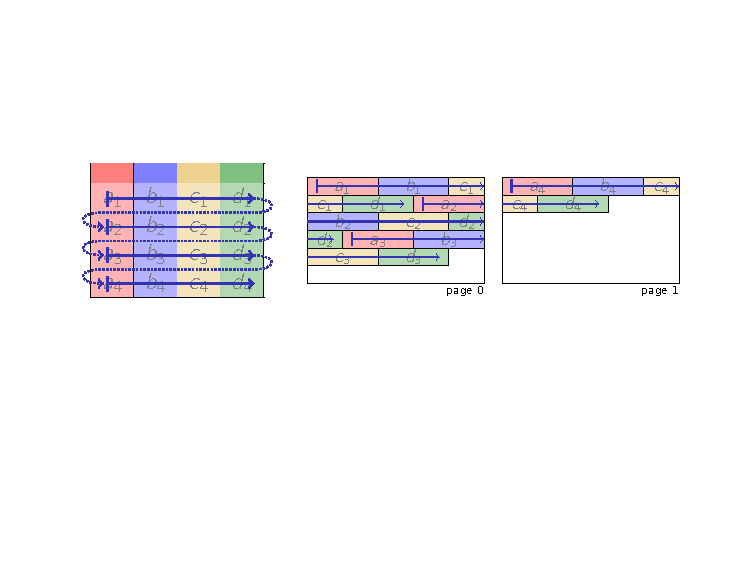
\includegraphics[scale=1.25]{images/rowstore}
\end{center}
\caption{Row-wise storage~\cite{JensDPMH}}
\label{fig:rowstore}
\end{figure}

Traditionally databases store their tables row-wise as seen in
Figure~\ref{fig:rowstore}. This means that a row is stored completely, then the
next row is stored adjacent to the last row and so on. When evaluating a
predicate on this rows all unused columns have to be skipped. Since the skipped
data is likely smaller than the minimum size of a data chunk that can be loaded
from DRAM by the CPU (a cacheline) a scan will load a lot of data that is not
used. But the far bigger issue with this layout is that it makes use of SIMD
much harder, as SIMD works best with homogeneous data. On current processors it
is unlikely that maximum performance can be achieved without using SIMD.

\begin{figure}[h] \begin{center}
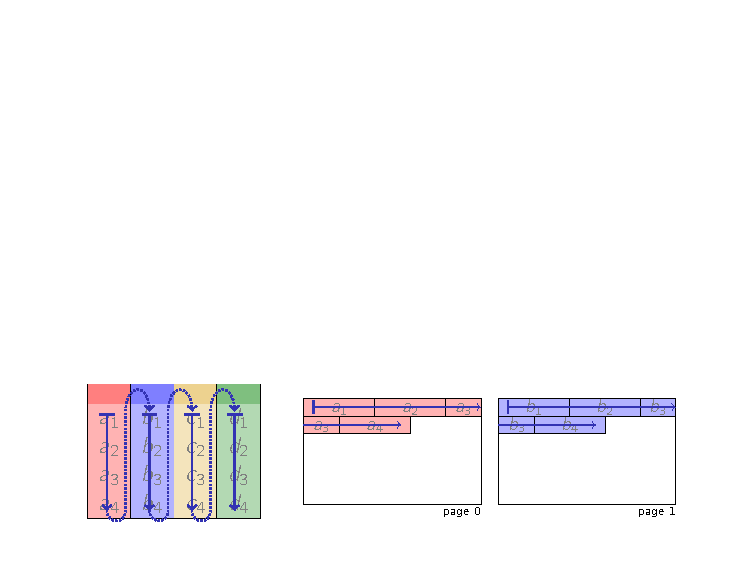
\includegraphics[scale=1.25]{images/colstore}
\end{center}
\caption{Column-wise storage~\cite{JensDPMH}}
\label{fig:colstore}
\end{figure}

The alternative to row-wise storage is to decompose the rows into individual
columns and store them as shown in Figure~\ref{fig:colstore}~\cite{copeland}.
This has several advantages over the row-wise format.

\begin{itemize}
  \item Less data is being fetched from memory during a scan. Columns not used
    in a scan can be ignored completely.
  \item SIMD is easily applied as all values in a column have the same format.
  \item More potential for compression as the elements in one column are often
    similar to each other.
\end{itemize}

The major downside of this format is fetching a row from a column store is more
complex than fetching one from a row store. After the row has been selected, all
columns have to be joined, this incurs at least a potentially random access for
every column. The column store trades scan performance for a slower access of
rows. Since the goal is to make scans as fast as possible this thesis will focus
on column stores.

\section{SIMD on Modern Hardware}

The focus of this section lies on the current 4th generation Intel Core
architecture. The basic observations are also applicable to any other current
architecture or SIMD instruction set, but the performance characteristics may
differ widely.

Intel has a long history supplying multimedia instruction sets:
\begin{description}
\item[MMX] The Multi Media eXtension made the start in 1997, supplying integer
instructions on 64 bit registers shared with the existing floating point unit.
\item[SSE] The Streaming SIMD Extension added a fully independent 128-bit
register set in 1999. SSE only supported floating point operations, SSE~2 added
the integer counterparts in 2001. SSE was extended with many different
instructions often catered towards operations commonly found in video codecs.
\item[AVX] The Advanced Vector eXtensions extend the registers introduced in
SSE to 256 bits. As with SSE, AVX provided only floating point operations and
AVX~2 added integer instructions. AVX also provides new encodings for all
existing SSE instructions using a three-operand form instead of the more
restricted two-operand form used by SSE. AVX instructions generally behave as
if working on two independent 128-bit registers instead of one large 256-bit
register, this makes operations that combine bits from the lower 128 bits with
bits from the upper 128 bits of the register more complex.
\item[AVX-512] AVX-512 is a new instruction set extending the AVX registers to
512 bits. While it contains interesting new operations that could be very
useful for implementing scans it was not available in general purpose CPUs at
the time this thesis was written.
\end{description}

Since AVX~2 is currently the latest available set of SIMD instructions on Intel
hardware it will be the focus of this thesis. It provides 16 256-bit registers
and integer operations on 32 8-bit, 16 16-bit, 8 32-bit or 4 64-bit values at a
time.

As a preliminary it is vital to understand how caches are organized on a
current Intel CPU. Since for a scan data will almost always be loaded freshly
from DRAM, cache levels are ignored here. The cache on any recent Intel CPU is
partitioned into cache lines of 64 bytes. This means that when reading data
from memory it does not matter if 1 byte or 32 bytes -- which is the maximum load
size in AVX~2 -- are read at a time and the whole cache line will be fetched from
DRAM.

A scan over an array of integers of size 8, 16, 32 or 64 bits can be
easily implemented in SSE or AVX as illustrated in
Figure~\ref{fig:simplecomparesse}. Here a greater than predicate is executed,
the \texttt{pcmpgt} instruction takes two vectors and sets the corresponding
element in a result vector to either all ones if the element in the first
vector is greater than the element in the second vector. Otherwise it is set to
zero. To generate a bit vector from this result the \texttt{movmsk} instruction
is used, which takes the most significant bit of every element in a vector and
sets the bit with the same number in a simple integer. In the example the
result of \texttt{movmsk} is $00111101$ in binary or $3d$ in hexadecimal.

\begin{figure}\center
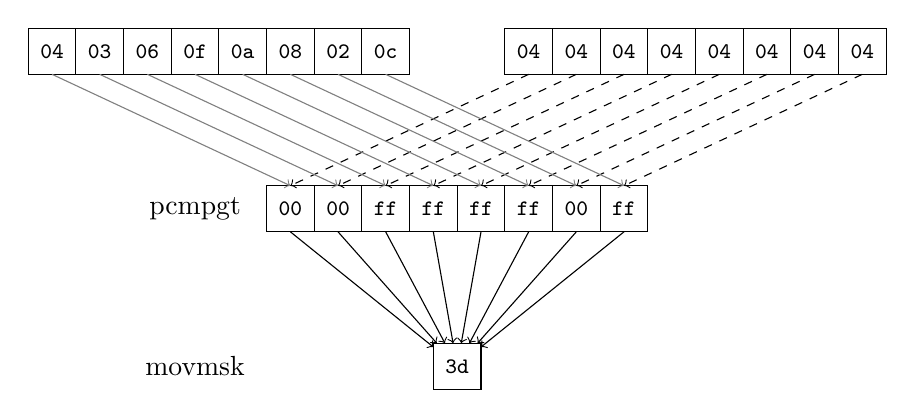
\begin{tikzpicture}[node distance=2cm]

\def\elemwidth{4ex};
\def\dotswidth{4ex};
\def\labelsepa{0.2cm};
\tikzset{simd element/.style={
    rectangle,
    draw,
    inner xsep=0.1ex,
    font=\footnotesize\ttfamily,
    minimum width=\elemwidth,
    minimum height=1.666em
}};

\foreach \val [count=\i] in {04, 03, 06, 0f, 0a, 08, 02, 0c} {
    \node[simd element] (src1\i) [
        xshift=(\i-1)*\elemwidth, outer sep=0] {\val};
}

\foreach \val [count=\i] in {04, 04, 04, 04, 04, 04, 04, 04} {
    \node[simd element] (src2\i) [
        xshift=(10+\i-1)*\elemwidth, outer sep=0] {\val};
}

\foreach \val [count=\i] in {00, 00, ff, ff, ff, ff, 00, ff} {
    \node[simd element, below of=src16] (src3\i) [
        xshift=(\i-1)*\elemwidth, outer sep=0] {\val};
}

\node[label, below of=src14] (pcmp) {pcmpgt};

\foreach \i in {1,...,8} {
    \path[->, color=gray] (src1\i.south) edge (src3\i.north);
    \path[->, dashed] (src2\i.south) edge (src3\i.north);
}

\node[simd element, below of=src34] (src4) [xshift=\elemwidth/2, outer sep=0] {3d};

\foreach \i in {1,...,8} {
    \path[->] (src3\i.south) edge (src4);
}

\node[label, below of=pcmp] (movmsk) {movmsk};
\end{tikzpicture}
\caption{Comparing two vectors and generating a bit vector in SSE}
\label{fig:simplecomparesse}
\end{figure}

\section{\simdscan{}}

\simdscan{} \cite{SIMD-Scan} takes the basic idea shown in
Figure~\ref{fig:simplecomparesse} and extends it to arbitrary bit widths. The
methodology is comparable to a normal compression format where data is first
decompressed in one step and then processed in another. The compression format
stores a set of fixed-size integers without any padding. For decompression those
individual integers have to distributed over the lanes of a SIMD vector. The
main achievement of \simdscan{} is an efficient decompression method for all of
the 32 bit cases from one bit to 32 bits. Due to limitations in Intel's vector
extensions, the performance of the bit case can vary though, with cases 8, 16 and
32 bit being trivial on SSE hardware as decompression is equivalent to a simple
copy here. Other bit widths require varying amounts of arithmetic and logic
operations to decompress. In practical implementations of \simdscan{} such as in
the in-memory database SAP HANA every bit case is implemented manually to
get an optimal sequence of instructions in a tight loop.

\vspace{.5cm}

\begin{figure}[h] \begin{center}
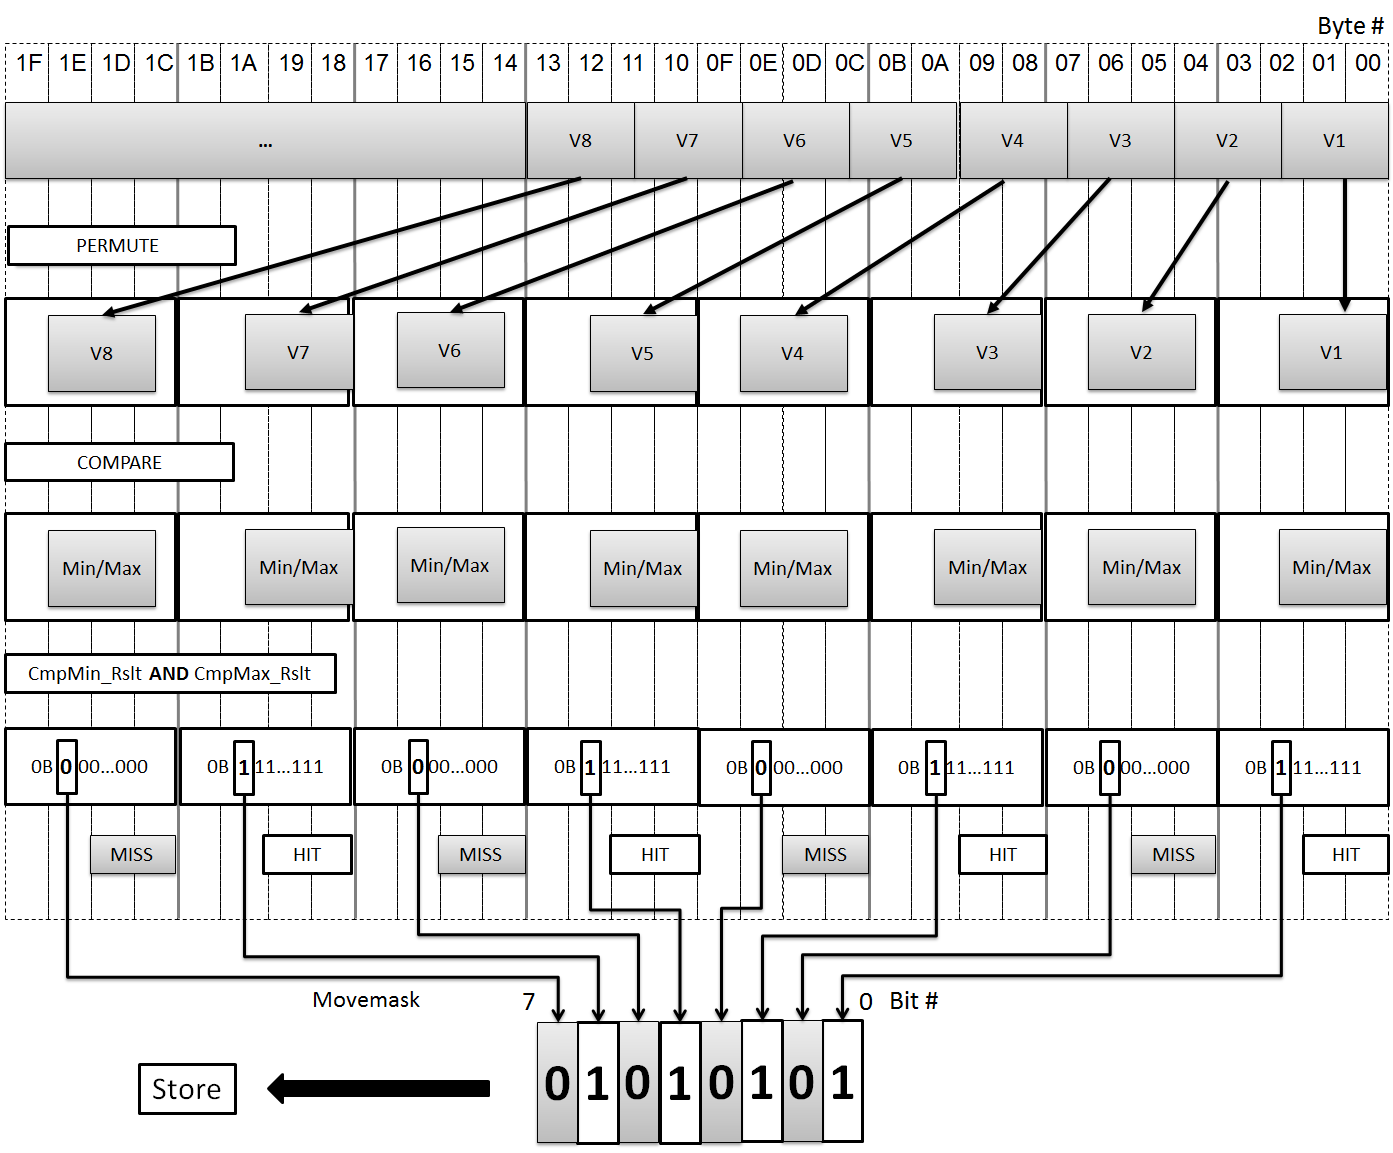
\includegraphics[scale=.3]{images/scan.png}
\end{center}
\caption{Vector comparison with \simdscan{}~\cite{AVX2-Scan}}
\label{fig:simdscan}
\end{figure}

The basic steps performed when evaluating a range predicate $\min < x < \max$
with \simdscan{} are shown in Figure~\ref{fig:simdscan}. The example uses a bit
width of 20 bits per word and a 256-bit vector register holding eight 32-bit
values.  In a first step eight values (160 bits) are loaded from the table and
permuted over the eight vector lanes. Because the permutation operation only
works on byte boundaries the result of this step is not aligned on the 32-bit
boundaries.  The next step would now be to shift the individual values to the
boundaries resulting in an aligned vector, but here a different approach is
taken. Since only comparisons are performed instead of shifting the values
loaded from the table, the reference constants $\min$ and $\max$ are shifted
before entering the main loop avoiding some work. Then the permuted values are
compared to the permuted $\min$ and $\max$ constants, yielding a bit vector
similar to the process shown in Figure~\ref{fig:simplecomparesse}. Because a
range predicate is evaluated, the two comparison results are combined with an AND
operation and turned into a bit vector using the \texttt{movemask} instruction.
This bit vector result is then written into the output buffer.

\simdscan{} has greatly benefited from new instruction set extensions such as
AVX~2 \cite{AVX2-Scan} and is likely to benefit from AVX~512 too, as more general
shuffle and compare instructions have been added, reducing the amount of
instructions needed for some bit widths.

As will be shown in Chapter~\ref{chapter:evaluation}, the \simdscan{} is bound by
memory bandwidth alone for almost any bit width when using AVX~2 on a modern
CPU. On Intel hardware this is a fairly new behavior that was not observed using
plain SSE \cite{AVX2-Scan} and required a lot of manual optimization. This also
means that \simdscan{} already has the best possible performance when all bits
of a column are read. There are three possible strategies to improve this.

\begin{itemize}
  \item Using a more complex compression scheme such as PFOR~\cite{PFOR} which
    tries to reduce the overall bit width by putting large numbers in a separate
    memory area and providing a reference to this table in the column. This
    still allows random access but requires a decoding step and trades
    memory bandwidth for performance when scanning data containing many large
    numbers.
  \item Using a variable-length encoding such as Simple-8~\cite{Simple8} or
    varint~\cite{varint} which store significantly fewer bits if an entry in the
    column is small. This complicates random access and makes fully utilizing
    SIMD harder, because SIMD instructions are usually only provided for
    fixed-size integers.
  \item Trying to abort the scan before all bits are read. This is possible by
    modifying the storage format and performing the comparison of a word on
    smaller chunks than the full word size.
\end{itemize}

The following sections focus on exiting the scan early, because this is most
likely to have the lowest overhead of the three methods.

\section{\emph{BitWeaving}}

\emph{BitWeaving} \cite{BitWeaving} is a new framework to further accelerate
scans by rearranging the bits scanned in memory for better performance. It comes
in two variants, a horizontal version, \emph{BitWeaving/H}, and a vertical
version, \bwv{}.

\begin{figure}[h] \begin{center}
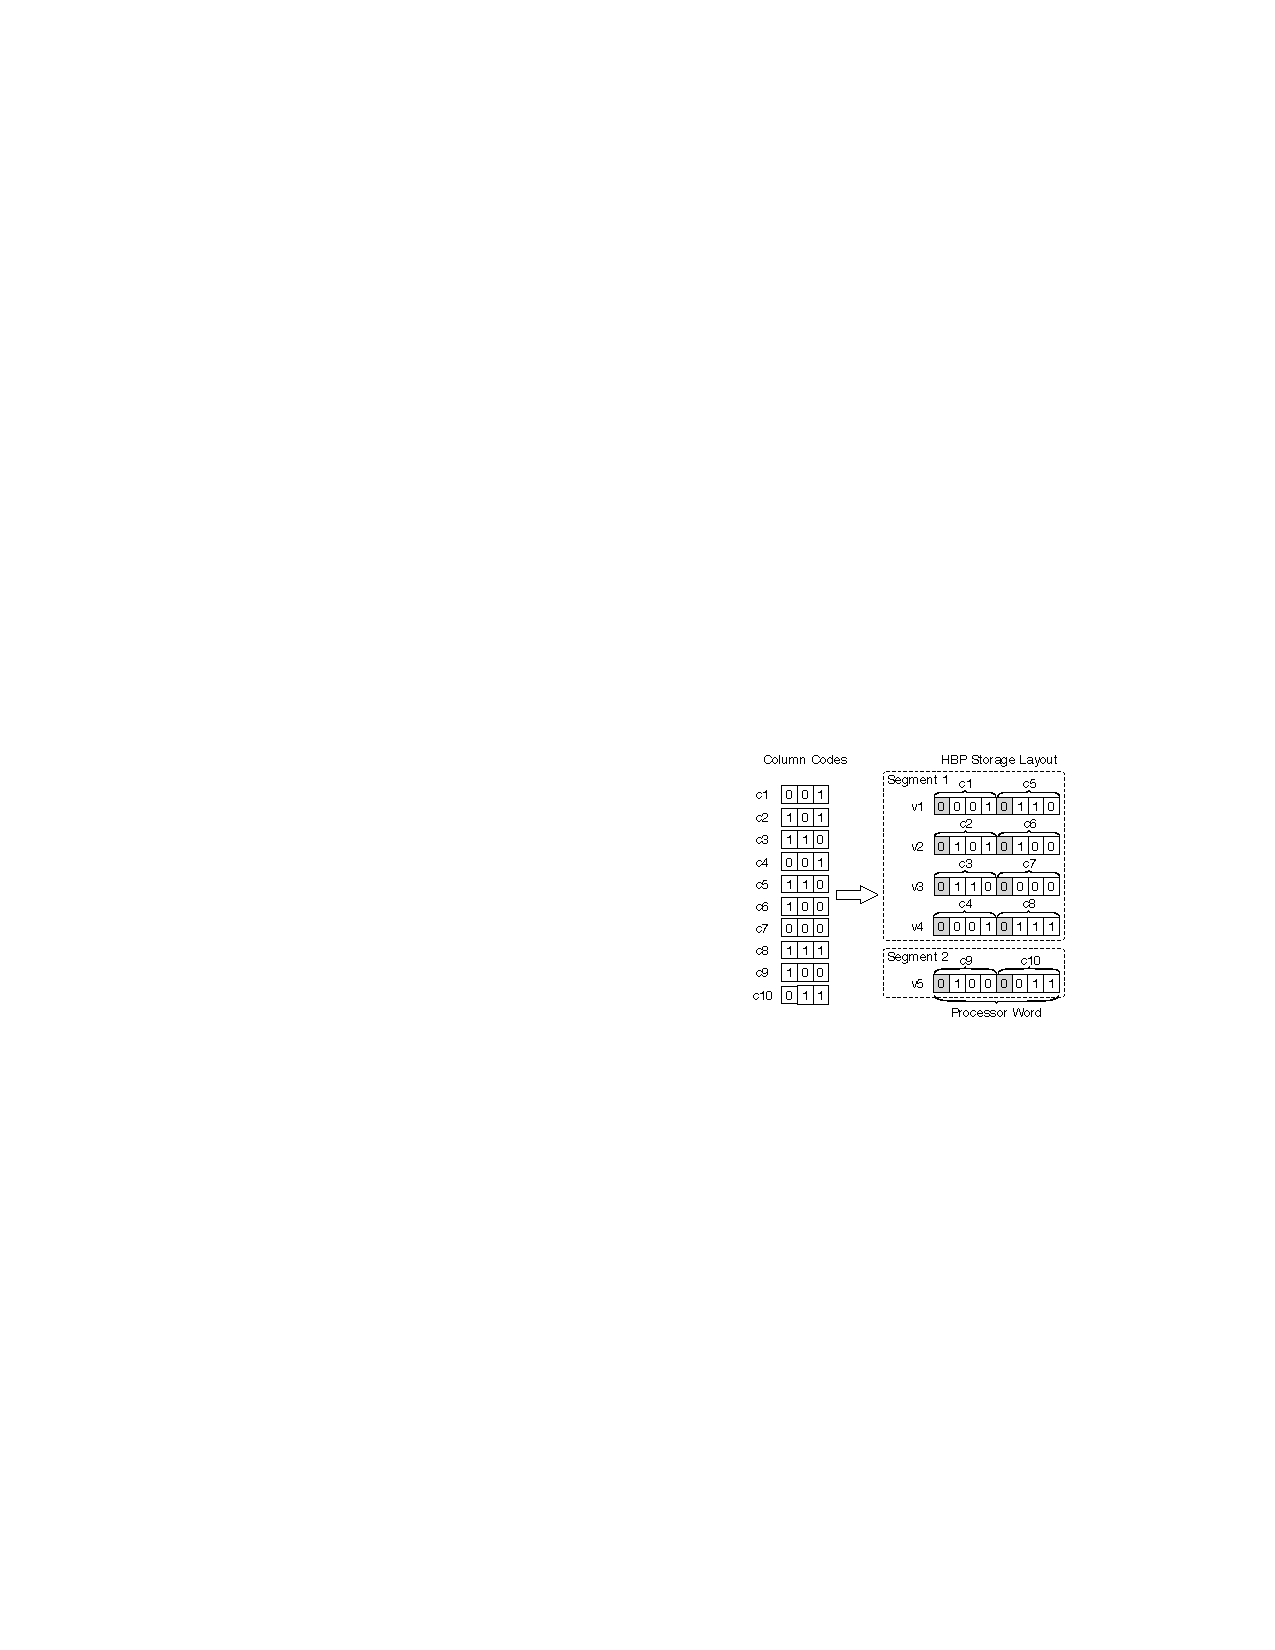
\includegraphics[scale=1.5]{images/bwh}
\end{center}
\caption{Storage layout of a horizontal bit packed format~\cite{BitWeaving}}
\label{fig:bwh}
\end{figure}

The horizontal form is based on ``SIMD within a register'' (SWAR) as first
described by Leslie Lamport in 1975 \cite{SWAR}. The data is stored
contiguously, similar to the format \simdscan{} uses, except that a stop bit is
added between every element, thus adding memory overhead. An example is shown in
Figure~\ref{fig:bwh}. To perform a scan on this data it is not decompressed, but
the arithmetic primitives used to do a comparison are decomposed and directly
applied to the compressed data. This approach is different from \simdscan{}.

As \emph{BitWeaving/H} provides no significant advantage over \simdscan{}, but
adds additional memory overhead it was not taken into consideration. Knuth
suggests in \cite{SWAR} that the additional bit can be avoided by adding more
arithmetic operations, it is however unlikely that this will make
\emph{BitWeaving/H} faster than \simdscan{}, the contrary is more likely.
\emph{BitWeaving/H} also has to read all the data for a scan.

Not reading all the data is the primary advantage of the other flavor of
\emph{BitWeaving}, \bwv{}. This format uses a vertical format first suggested in
\cite{oneill}. The individual bits of a word in the column are no longer stored
together, but distributed over many words. In memory this means that the most
significant bits of all words are stored first, followed by the second-most
significant bits and so on as seen in Figure~\ref{fig:bwv}. Scans are still
implemented using a SWAR method on a bit-wise level. The difference is now that
for a comparison operation the scan of a word is aborted after a mismatch occurs
for the first time. Any additional bits do not have to be read anymore. This
behavior is called early pruning or early exiting.

\begin{figure}[h] \begin{center}
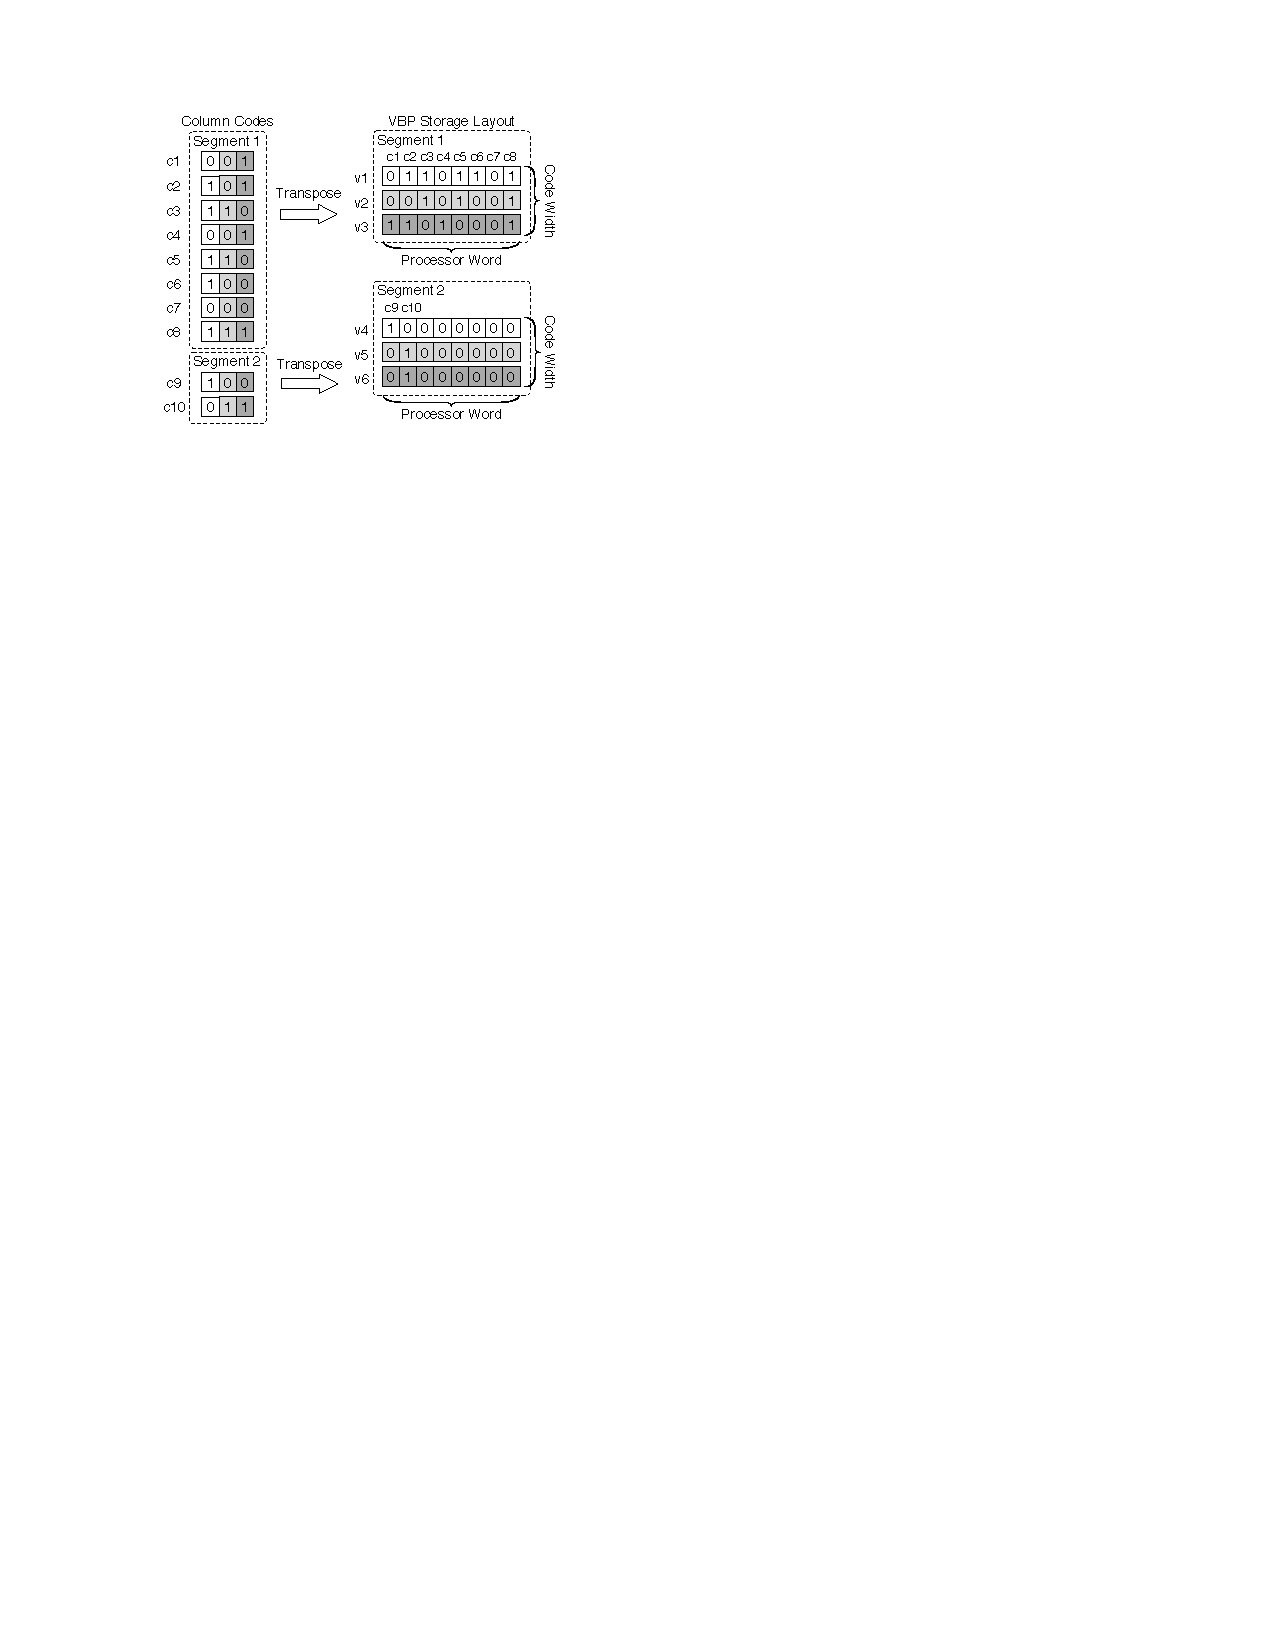
\includegraphics[scale=1.5]{images/bwv}
\end{center}
\caption{Storage layout of a vertical bit packed format~\cite{BitWeaving}}
\label{fig:bwv}
\end{figure}

To derive a performance advantage out of the memory that is not read anymore the
column is partitioned into a fixed amount of groups. This can be imagined as
first storing the four most significant of all words first, in the vertical
format. This forms the first partition or group. Then the fifth to eighth
significant bits are stored in the next group and so on. Early pruning is
performed after a full group is processed, so the processor can take advantage of
the sequential access without any interruption. This also reduces the likeliness
of mispredicted branches as the total number of early pruning branches is
reduced.

The major downside of this vertical format is the same that was seen when
switching from row-wise to column-wise storage. Again, this is a trade-off
between scan performance and the amount of work necessary to extract a row from
the storage. As the bits of a single value are now distributed over many memory
locations, reading it becomes a lot slower.
\newpage
\section{\bs{}}

\bs{} \cite{ByteSlice} can be seen as a hybrid between vertical and horizontal
bit packing formats. It is very similar to the \bwv{} format, but does not
distribute individual bits over multiple locations. It only distributes bytes.
Intel's SIMD extensions have very efficient instructions for byte-level
comparisons and permutations, so this avoids complexity in the scan loop.

This byte-level vertical format has several advantages over the bit-level
vertical format. Packing and unpacking \bs{}d data only has to touch one eighth
of the memory locations \bwv{} has to access. Furthermore, moving bytes in a
vector register for packing and unpacking can be done using shuffle instructions
in most SIMD instruction sets. Bit-level shuffling is usually not available.
This allows very fast access of individual values without the high overhead in
the \bwv{} format while still providing early pruning opportunities.

When comparing early pruning, it might seem like \bwv{} provides better pruning
opportunities as aborting is possible after every bit in theory. \bs{} can only
prune after quantities of eight bits have been processed. This is only partially
true though, because \bs{} contains fewer values per vector word, so early pruning
is more likely to occur, a single value in a vector word in either format can
prevent early exiting. The grouping in \bwv{} also reduces the early pruning
opportunities, but this can also be applied to \bs{}. However, \bs{} group sizes
are always a multiple of eight.

The storage of bytes also comes at a cost of flexibility. \bwv{} can easily
store any bit width with no memory lost to overhead bits. \bs{} is limited to
multiples of eight, all other bit widths add more complexity. One solution is to
pad to the next multiple of eight with zeros. For example a column of eleven bit
values is padded to 16-bit values, adding three bits of overhead as shown in
Figure~\ref{fig:bseleven}. In the worst case this can add up to seven bits of
overhead per value. This is clearly a disadvantage when the scan is limited by
memory bandwidth. Another solution would be to store as many bytes as possible
and switch to the \bwv{} format for the remaining bits. For eleven bit values
this would be one byte in \bs{} and three bit in \bwv{}. This also has zero
memory overhead, but increases the complexity of the scan by splitting it into
two stages.

\begin{figure}[h] \begin{center}
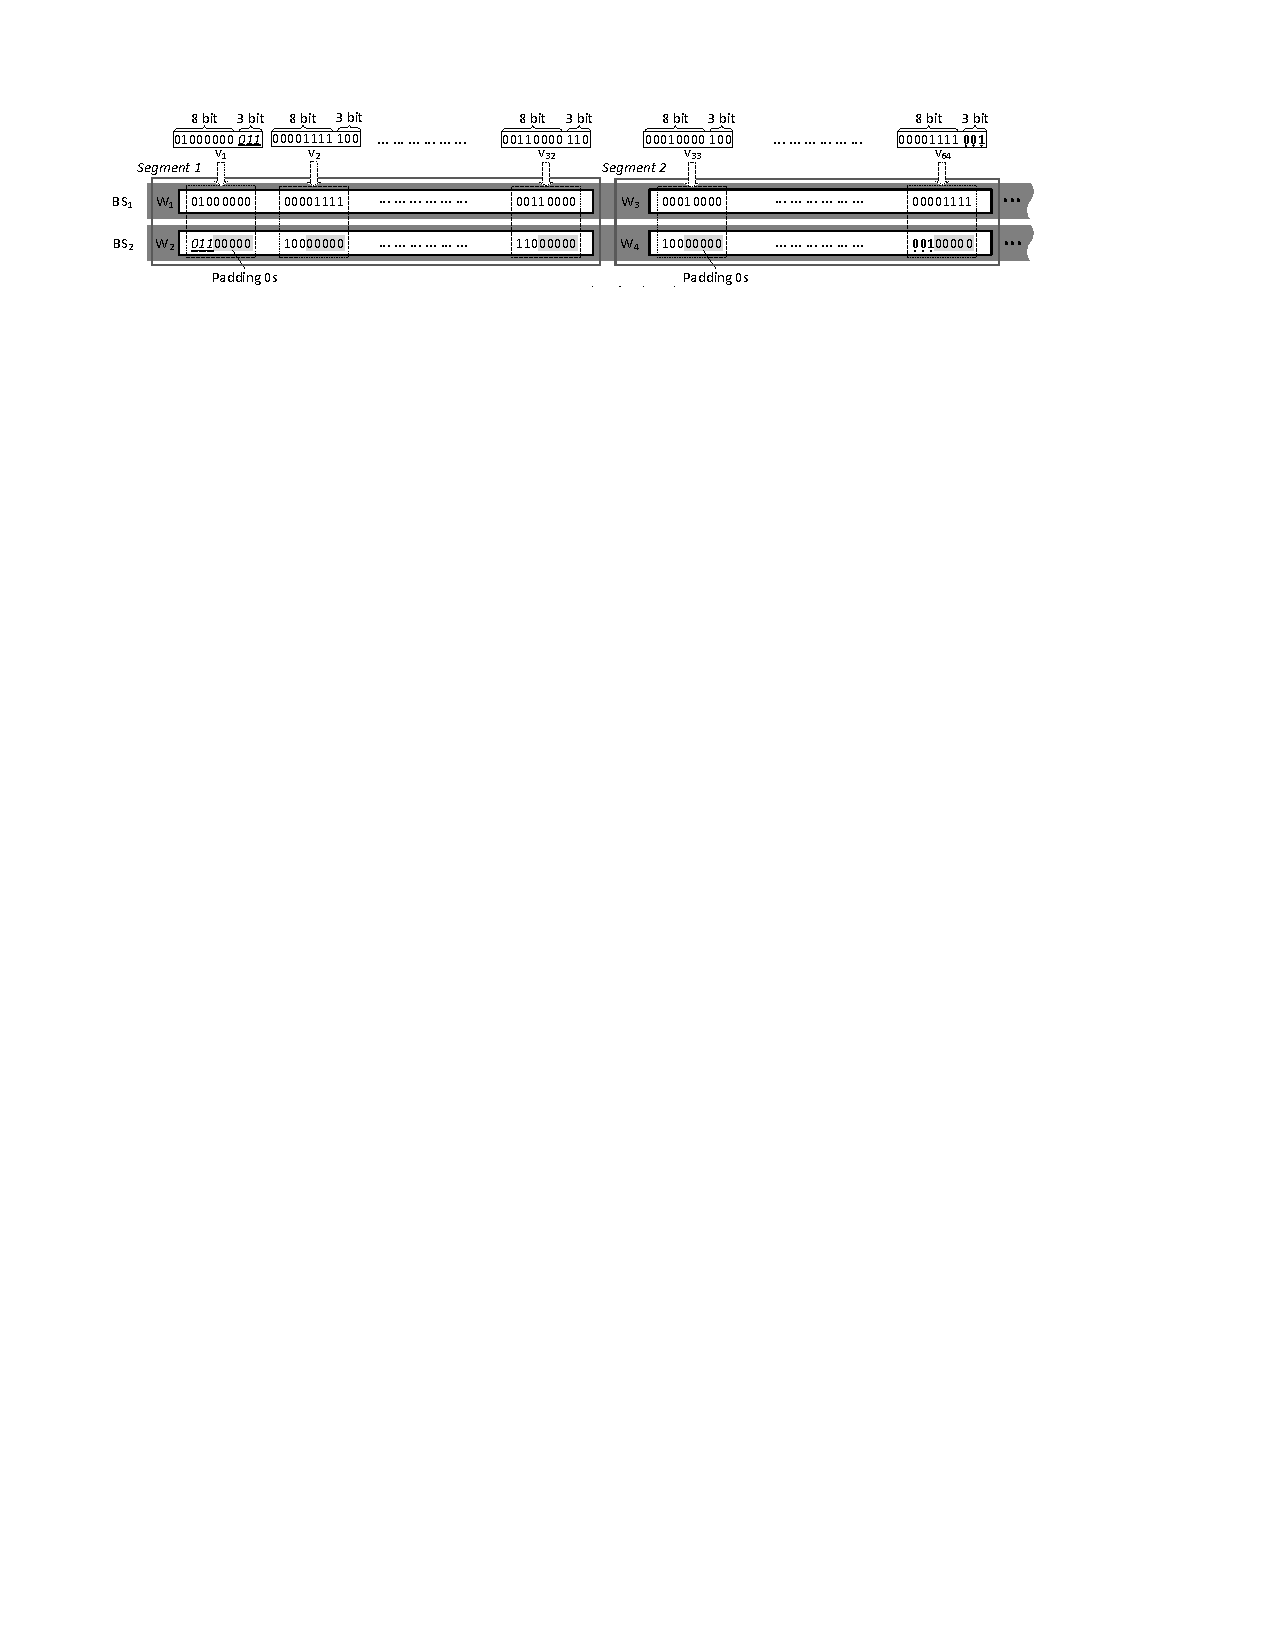
\includegraphics[scale=1]{images/bytesliceelevenbits}
\end{center}
\caption{Storage layout eleven bit values in \bs{} using zero padding~\cite{ByteSlice}}
\label{fig:bseleven}
\end{figure}

\section{Summary}

In this chapter we have seen a basic overview of memory and SIMD instructions on
modern hardware and methods to perform scans on in-memory column stores.
\simdscan{} is one method for scans that works very well on modern hardware,
being only limited by the bandwidth from memory to the CPU core. \bwv{} and
\bs{} are two techniques that look very promising as they are likely just as
bound by memory bandwidth as \simdscan{} and their scans are not more complex in
terms of instructions executed. However, these methods can extract additional
advantages by using a more sophisticated memory layout to avoid reading all bits
from memory and thus saving precious memory bandwidth.

\bwv{} and \bs{} are very similar in their basic idea and behavior, but differ in
details. This affects the number of branches executed, the probability of early
pruning and the complexity of bringing data into the scan representation and
vice-versa. This justifies a separate analysis of both approaches.

In the rest of the thesis we will evaluate how this early exiting performs when
doing a scan both in theory and with practical benchmarks. In contrast to
\simdscan{} performance analysis now contains a probabilistic component
depending on the input data.
